%%%%%%%%%%%%%%%%%%%%%%%%%%%%%%%%%%%%%%%%%
% baposter Portrait Poster
% LaTeX Template
% Version 1.0 (15/5/13)
%
% Created by:
% Brian Amberg (baposter@brian-amberg.de)
%
% This template has been downloaded from:
% http://www.LaTeXTemplates.com
%
% License:
% CC BY-NC-SA 3.0 (http://creativecommons.org/licenses/by-nc-sa/3.0/)
%
%%%%%%%%%%%%%%%%%%%%%%%%%%%%%%%%%%%%%%%%%

%----------------------------------------------------------------------------------------
%   PACKAGES AND OTHER DOCUMENT CONFIGURATIONS
%----------------------------------------------------------------------------------------

\documentclass[a0paper,portrait,colspacing]{baposter}

\usepackage[font=small,labelfont=bf]{caption} % Required for specifying captions to tables and figures
\usepackage{booktabs} % Horizontal rules in tables
\usepackage{relsize} % Used for making text smaller in some places
\usepackage{url}
\usepackage{floatrow}

\graphicspath{{figures/}} % Directory in which figures are stored

\definecolor{bordercol}{RGB}{0,0,256} % Border color of content boxes
\definecolor{headercol1}{RGB}{100,200,200} % Background color for the header in the content boxes (left side)
\definecolor{headercol2}{RGB}{100,120,200} % Background color for the header in the content boxes (right side)
\definecolor{headerfontcol}{RGB}{0,0,0} % Text color for the header text in the content boxes
\definecolor{boxcolor}{RGB}{250,250,250} % Background color for the content in the content boxes

\begin{document}

\background{ % Set the background to an image (background.pdf)
\begin{tikzpicture}[remember picture,overlay]
\draw (current page.north west)+(-2em,2em) node[anchor=north west]
{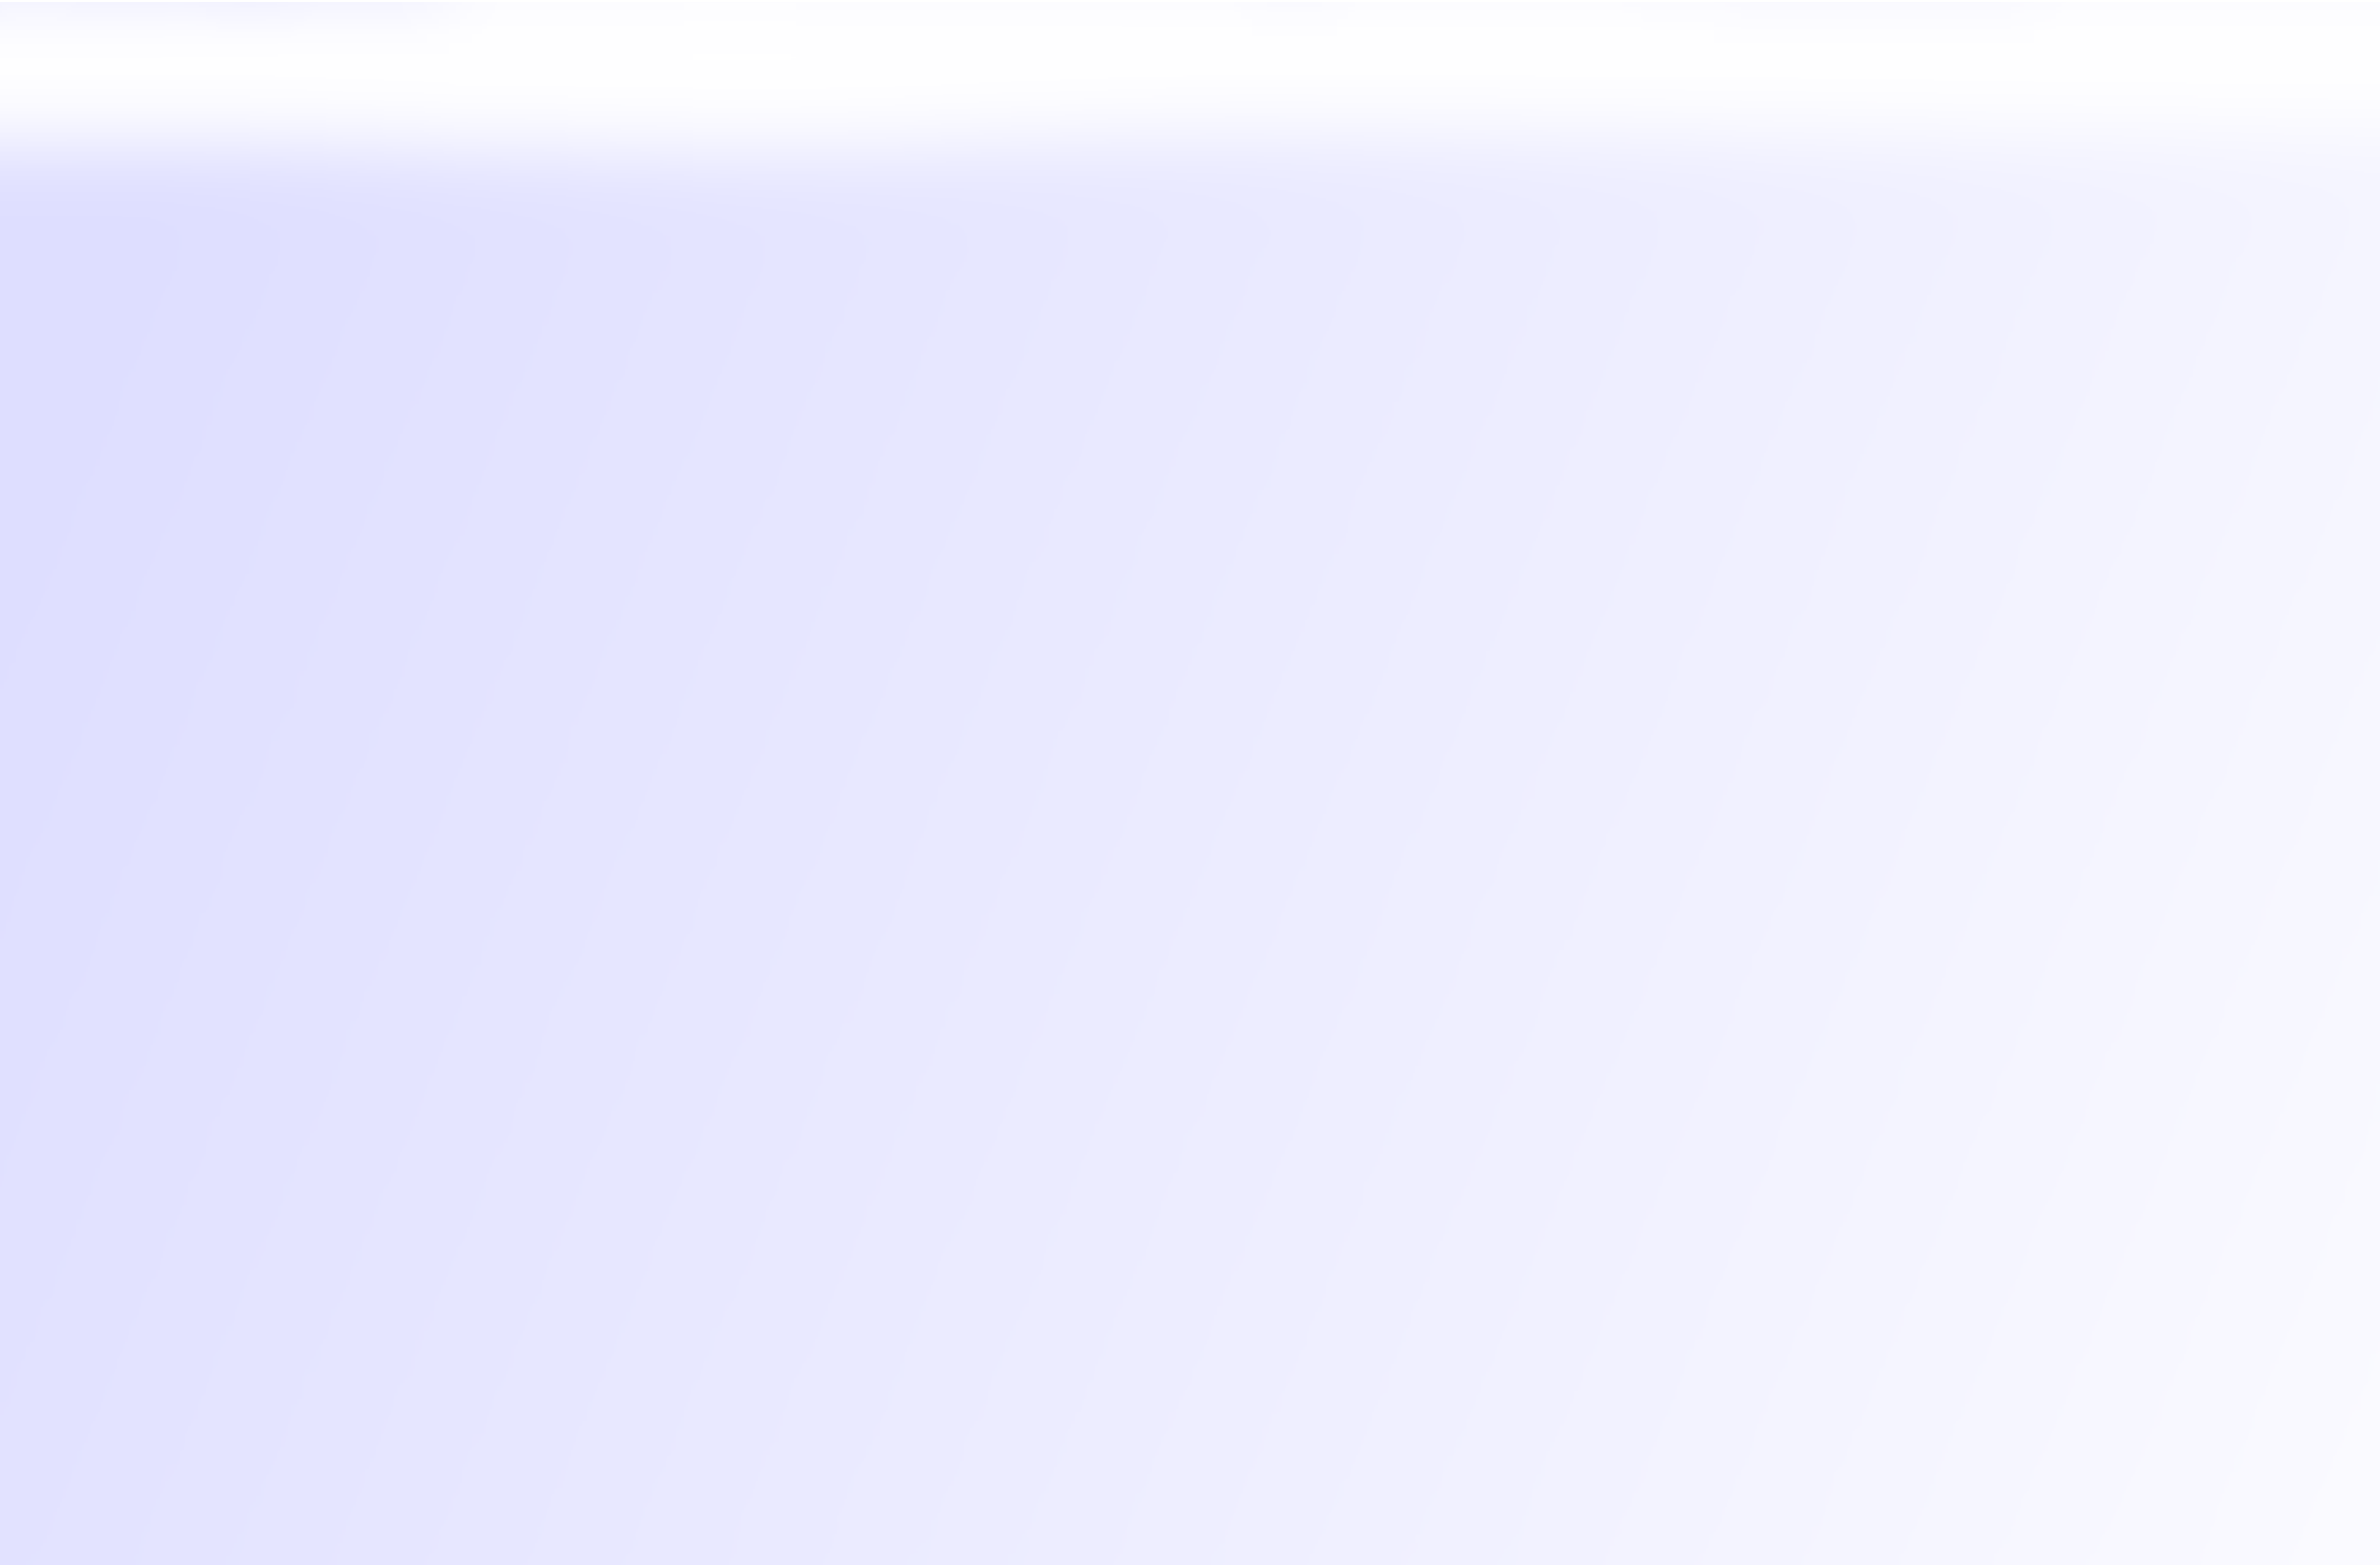
\includegraphics[height=1.1\textheight]{background}};
\end{tikzpicture}
}

\begin{poster}{
grid=false,
borderColor=bordercol, % Border color of content boxes
headerColorOne=headercol1, % Background color for the header in the content boxes (left side)
headerColorTwo=headercol2, % Background color for the header in the content boxes (right side)
headerFontColor=headerfontcol, % Text color for the header text in the content boxes
boxColorOne=boxcolor, % Background color for the content in the content boxes
headershape=roundedright, % Specify the rounded corner in the content box headers
headerfont=\Large\sf\bf, % Font modifiers for the text in the content box headers
textborder=rectangle,
background=user,
headerborder=open, % Change to closed for a line under the content box headers
boxshade=plain
}
{
\includegraphics[scale=0.20]{SwarmathonLogo.png}}  %%%Added left logo
%
%----------------------------------------------------------------------------------------
%   TITLE AND AUTHOR NAME
%----------------------------------------------------------------------------------------
%
{\sf\bf\textsc{The Deterministic Spider: A Benchmark for Evaluating Efficiency of Swarm Search}} % Poster title
{Linh T. Tran, G. Matthew Fricke, Joshua P. Hecker, Antonio D. Griego, \& Melanie E. Moses\\ % Author names
{\smaller litran11794@unm.edu, matthew@fricke.co.uk, jhecker@cs.unm.edu, deano505@unm.edu, and melaniem@cs.unm.edu}} % Author email addresses
{
\includegraphics[height=4.5em]{UNMLogoVertColor.jpg}} % University/lab logo

%----------------------------------------------------------------------------------------
%   MOTIVIATION AND CONTRIBUTION
%----------------------------------------------------------------------------------------

\headerbox{Motivation and Contribution}{name=motiveandcontribution,column=0,row=0}{
\begin{itemize}
% \setlength{\itemindent}{-1em}
\item Swarm Robotics uses simple, scalable, inexpensive, and flexible approaches that emulate biological systems \cite{NasaSwarmathon}.
\item There is no standard to compare the efficiency of foraging search algorithms. 
\item \textbf{This research establishes a benchmark to compare efficiency of multi-robot foraging algorithms.}
\end{itemize}
%------------------------------------------------
This analysis compares the DSA against a stochastic search, Central Place Foraging Algorithm \cite{Hecker&Moses15Beyond}. We use a single robot and assume that the robot has perfect sensors and the environment is free of obstacles.\\ 
%------------------------------------------------
\\\textbf{Main contributions:}\\
A \textbf{benchmark algorithm} that allows evaluation of the efficiency of complex search algorithms.
}

% %----------------------------------------------------------------------------------------
% %   MATERIALS AND METHODS
% %----------------------------------------------------------------------------------------

% \headerbox{Materials and Methods}{name=methods,column=0,below=motiveandcontribution}{

% \begin{description}
% \item[ER1] Sed a orci non ipsum posuere placerat. Nunc in mi augue, a adipiscing massa. Donec dapibus gravida odio, condimentum convallis urna.\item[ER2] Nullam sagittis cursus neque, sit amet mollis elit auctor in. Etiam sed lectus a nulla rhoncus interdum a tempus nunc. Sed at eleifend purus.
% \end{description}

% Nullam sollicitudin lobortis urna quis varius. Nullam sagittis blandit diam, $DN = G_t(V_t,E_t)$, risus $E_t \subseteq V_t \times V_t$ ($\forall t \geq 0$). vel tortor justo, $G_0$, quis malesuada lorem.

% \begin{equation}
% \cos^3 \theta =\frac{1}{4}\cos\theta+\frac{3}{4}\cos 3\theta
% \label{eq:refname}
% \end{equation}

% Vivamus porta lacus et lectus \textbf{porta lacus}. Pellentesque habitant morbi tristique senectus et netus et malesuada fames ac turpis. torte $G_t$ hac millis \textbf{plates} Idk 
% }

%----------------------------------------------------------------------------------------
%   CONCLUSION
%----------------------------------------------------------------------------------------

\headerbox{Conclusion}{name=conclusion,column=0,below=motiveandcontribution}{

\indent For a single robot,
\begin{itemize}
\item \textbf{DSA is more efficient in finding randomly distributed food because it is a pre-planned exhaustive search that eliminates repeated steps.} 
\item \textbf{However, the DSA is only marginally better at finding tags in clustered environments.}
\item \textbf{The efficiency of the CPFA is less variable than the DSA.}\\
\end{itemize}
%------------------------------------------------
% \begin{center}
% \vspace{-1em}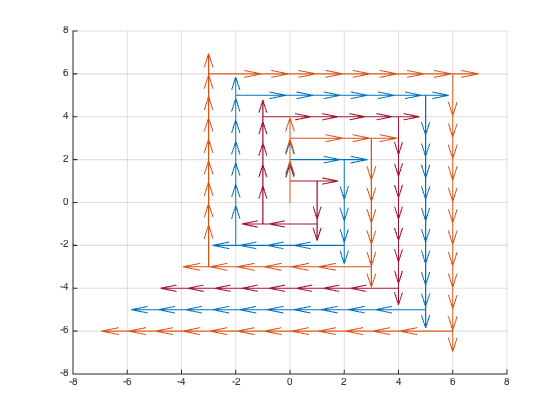
\includegraphics[width=5cm]{MultiRobot.png}\vspace{-1em}
% \captionof{figure}{Multiple robots performing the DSA.}
% 
\includegraphics[scale=0.20]{SwarmathonLogo.png}
% \end{center}
%------------------------------------------------
\indent Our future work will test our prediction that DSA is a reliable and efficient search algorithm for foraging swarms without error, but the CPFA is superior given large numbers of robots with localization error.\vspace{1em}
%------------------------------------------------
}

%----------------------------------------------------------------------------------------
%   REFERENCES
%----------------------------------------------------------------------------------------

\headerbox{References}{name=references,column=0,below=conclusion}{

% \smaller % Reduce the font size in this block
\renewcommand{\section}[2]{\vskip 0.05em} % Get rid of the default "References" section title
\nocite{*} % Insert publications even if they are not cited in the poster

\bibliographystyle{unsrt}
\bibliography{sample} % Use sample.bib as the bibliography file
}

% % %----------------------------------------------------------------------------------------
% % %   ACKNOWLEDGEMENTS
% % %----------------------------------------------------------------------------------------

\headerbox{Source Code}{name=sourcecode,column=0,below=references, above=bottom}{
 \noindent Project source code is available at: \\\vspace{1em}\url{https://github.com/BCLab-UNM} \\
 \noindent Project information, including iAnt build instructions and related work, is available at: \\
  \small \url{http://sites.google.com/site/unmantbot/}.
} 

%----------------------------------------------------------------------------------------
%   METHODS
%----------------------------------------------------------------------------------------

\headerbox{Methods}{name=methods,span=2,column=1,row=0}{ % To reduce this block to 1 column width, remove 'span=2'
Both aggregate food items to a fixed central location.
\begin{itemize}
\item DSA: Collects food systematically, eliminates revisited tracks, and uses a pre-determined search pattern, but relies on precise planning for robot location.
\item CFPA: Recruits robots to large clusters, uses probabilistic communication, and reduces computation and localization planning, but robots may repeatedly search the same location. 
\end{itemize}
We ran each algorithm 50 times for 1 hour real time trials, for multiple resource placements. We observed the number of resources collected per hour in random, power law, and clustered food distributions.\\
%------------------------------------------------
\begin{tabular*}{\linewidth}{*{3}{@{}p{0.32\linewidth}@{}}}
    {\hfill{}\large \hspace{-2em}\textbf{Random} \hfill{}} & {\hfill{} \large \textbf{Power Law} \hfill{}} &  {\hfill{} \large \hspace{4em}\textbf{Clustered} \hfill{}}
  \end{tabular*}
%------------------------------------------------
\hspace{500pt}
\hspace{50pt}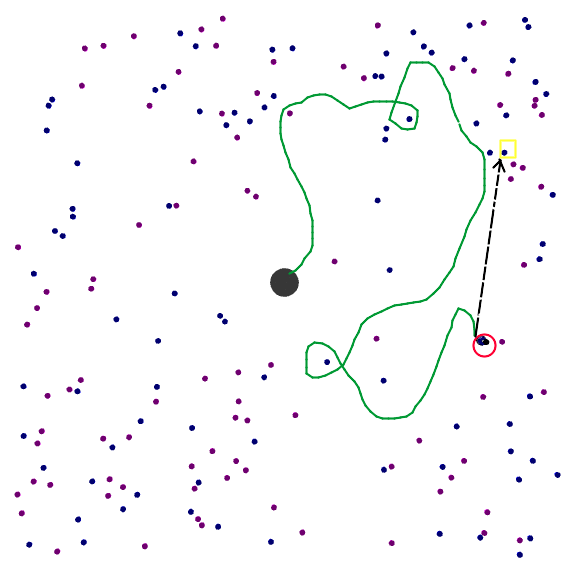
\includegraphics[width=0.25\linewidth,height=3cm]{RandomEnvr.png}
\hspace{50pt}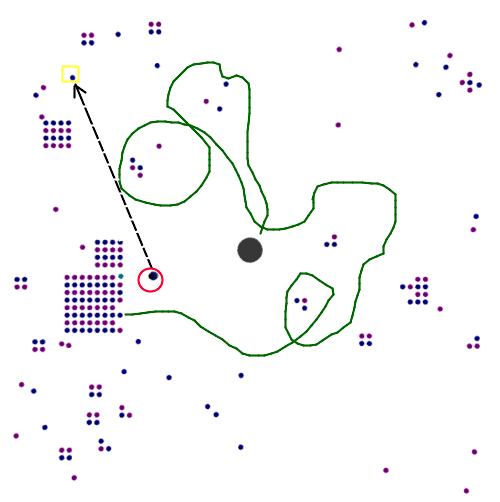
\includegraphics[width=0.25\linewidth,height=3cm]{PowerLawEnvr.png}
\hspace{50pt}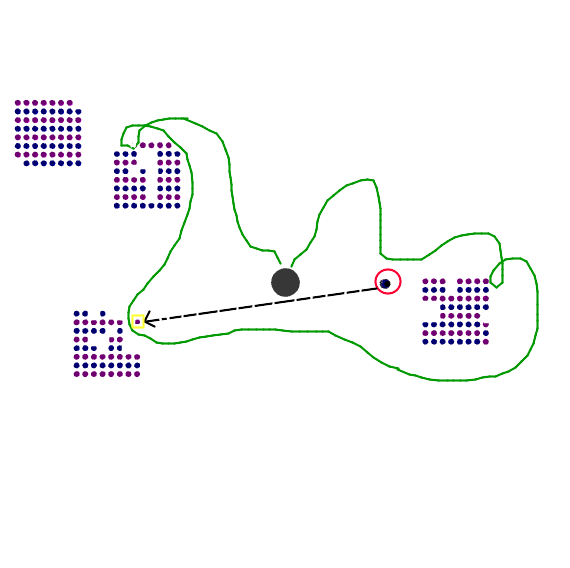
\includegraphics[width=0.25\linewidth,height=3cm]{ClusterEnvr.png}
\captionof{figure}{A path of an single robot retrieving a single seed (CPFA).}
%------------------------------------------------
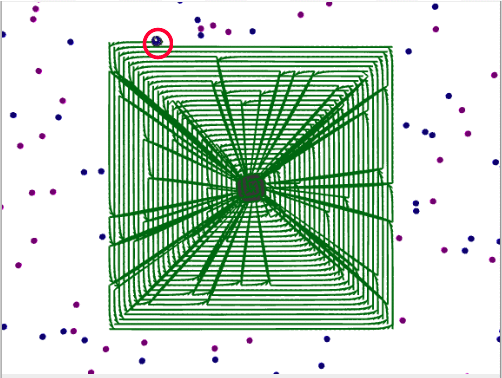
\includegraphics[width=0.25\linewidth]{RandomResults.png}
\hspace{50pt}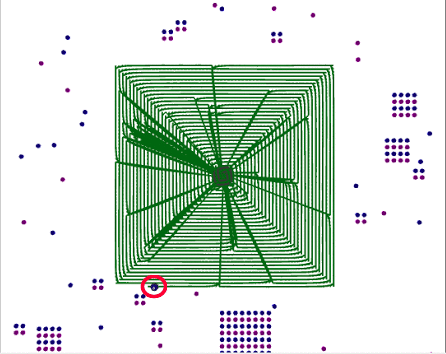
\includegraphics[width=0.25\linewidth]{PowerLawResults.png}
\hspace{50pt}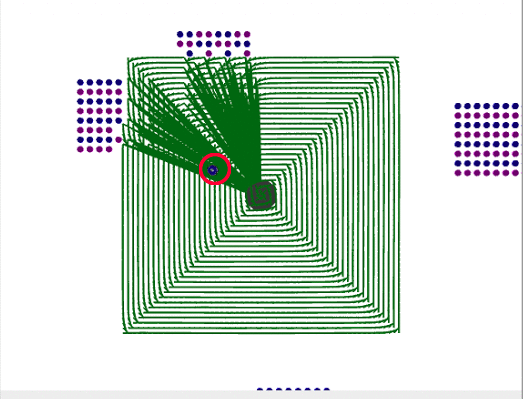
\includegraphics[width=0.25\linewidth]{ClusterResults.png}
\captionof{figure}{The full path of a single robot collecting for 60 minutes (DSA).}
}

%----------------------------------------------------------------------------------------
%   RESULTS 
%----------------------------------------------------------------------------------------

\headerbox{Results}{name=results,span=2,column=1,below=methods,above=bottom}{ % To reduce this block to 1 column width, remove 'span=2'

% \floatbox[{\capbeside\thisfloatsetup{capbesideposition={right,center},capbesidewidth=5.5cm}}]{figure}[\FBwidth]
% {\caption{Displays the percentage of improvement of DSA to the CPFA}\label{fig:test}}
% {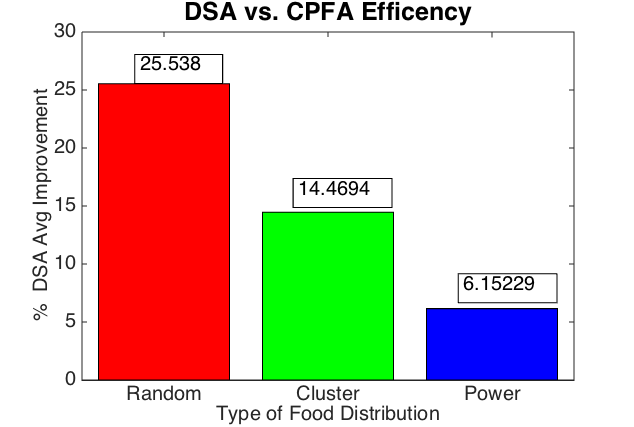
\includegraphics[width=5cm]{CPFAvsDSABar.png}}
%------------------------------------------------
% Our results reveal that: 

%------------------------------------------------
% \begin{center}
% % \includegraphics[scale=0.4]{CPFAvsDSA.png}
% 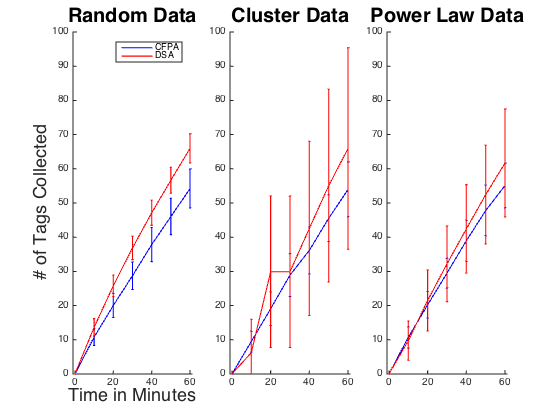
\includegraphics[scale=0.4]{CPFAvsDSALine.png}
% \captionof{figure}{Displays the standard and mean comparison of the CPFA and DSA with a single robot.}
% \end{center}
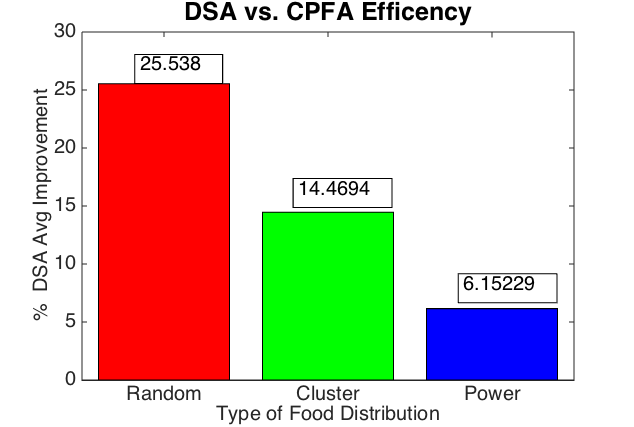
\includegraphics[width=0.35\linewidth]{CPFAvsDSABar.png}
\hspace{25pt}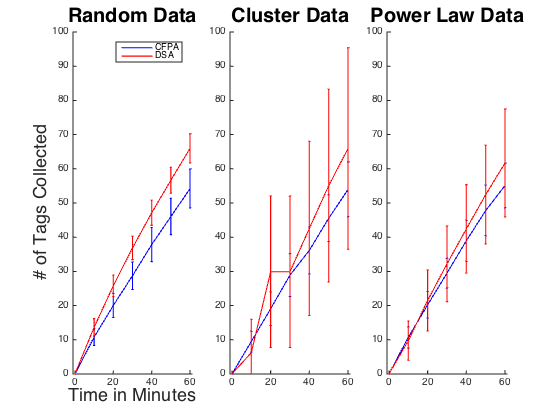
\includegraphics[width=7cm,height= 5.5cm]{CPFAvsDSALine.png}\par
\captionof{figure}{Displays the percentage, standard, and mean improvement of the DSA to the CPFA with a single robot. The left figure shows the overall average improvement percentage.}
\begin{itemize}
\item A single robot performing the DSA does $25.5\%$ better when collecting randomly distributed resources than the CPFA. 
\item Given that all data is statistically distinguishable, the improvement in the DSA for the Power law and Clustered environments are relatively small compared to Random.
\item The DSA produces more variable results due to its dependence on food placement. In comparison, the CPFA produces more predictable results, despite using probabilistic communication.
\end{itemize}
\textbf{Multiple Robots in the DSA}\vspace{-1em}
%------------------------------------------------

\floatbox[{\capbeside\thisfloatsetup{capbesideposition={left,center},capbesidewidth=5cm}}]{figure}[\FBwidth]
{\caption{The paths of 3 robots performing the DSA (Results TBA).}}
{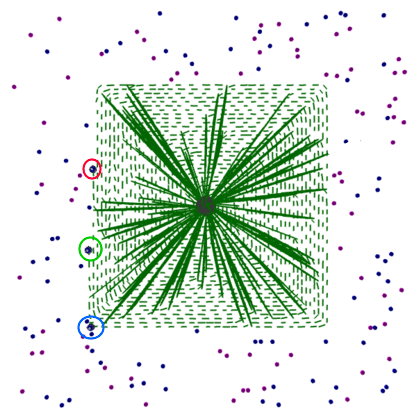
\includegraphics[width=5cm]{3RobotsDSA.png}}
}
%----------------------------------------------------------------------------------------

\end{poster}

\end{document}